\chapter{Atom Hidrogen}\label{ch:b3:hydrogen-atom}

Sembilan persepuluh atom di semesta adalah hidrogen: satu proton yang
menahan satu elektron, satu-satunya atom yang dapat diselesaikan fisika
secara eksak --- sekaligus kunci yang membuka semua atom lainnya. Teori
kuantum lama pada \cref{ch:b3:hamiltonian-mechanics} menerka energinya;
perangkatnya kini tersedia untuk \emph{menurunkannya}: potensial Coulomb
masuk ke \omterm{prop:b3:schrodinger-three-dimensions:swave}{persamaan radial} bab lalu, dan keluarlah aras
$-E_{\text{I}}/n^2$, \omterm{thm:b3:hydrogen-atom:levels}{jejari Bohr}, kulit dan subkulit tabel berkala
kimia, serta deret spektrum yang dibaca para astronom dalam tiap nebula.
Penyelesaian yang sama, setelah diskalakan ulang, memerikan helium
terionkan, atom muonik, positronium, dan ``atom'' elektron--lubang di
dalam semikonduktor; diregangkan sampai $n
\approx 100$ ia memerikan atom Rydberg selebar setengah mikrometer, yang
bisikan radionya memetakan awan terionkan Galaksi dan yang interaksinya
kini menggerakkan komputer kuantum.
% NOTE: full radial solutions (Laguerre) admitted; ground state solved
% exactly; emphasis on scaling laws and applications.

\section{Soal Coulomb terselesaikan}

\begin{theorem}[Aras hidrogen]\label{thm:b3:hydrogen-atom:levels}
\index{atom hidrogen}\index{bilangan kuantum utama}\index{jejari Bohr}
Untuk $V(r) = -e^2/4\pi\varepsilon_0 r$ (tuliskanlah $k = e^2/4\pi
\varepsilon_0$), keadaan terikatnya dilabeli $(n, l, m)$ dengan
\[
E_n = -\frac{E_{\text{I}}}{n^2} , \qquad
E_{\text{I}} = \frac{m_{\text{e}}k^2}{2\hbar^2} = \qty{13.6}{eV} ,
\qquad n = 1, 2, 3, \dots
\]
dan, untuk tiap $n$, bilangan orbitalnya $l = 0, 1, \dots, n-1$ serta
$m = -l, \dots, l$. Panjang alaminya adalah \omterm{thm:b3:hydrogen-atom:levels}{jejari Bohr} $a_0 =
\hbar^2/m_{\text{e}}k = \qty{52.9}{pm}$; keadaan dasarnya adalah
\[
\psi_{100} = \frac{1}{\sqrt{\pi a_0^3}}\;\eu^{-r/a_0} .
\]
Energinya bergantung pada $n$ \emph{saja}: dengan mencacah $m$ dan
$l$-nya, aras $n$ berdegenerasi $n^2$ kali (dilipatduakan oleh spinnya,
\cref{ch:b3:spin-two-level}) --- jauh melampaui degenerasi $(2l+1)$ kali
yang dijelaskan keisotropannya.
\end{theorem}

\begin{proof}[Bukti sebagian]
Untuk keadaan dasarnya, cobalah $u = Cr\,\eu^{-r/a}$ dalam \omterm{prop:b3:schrodinger-three-dimensions:swave}{persamaan
radialnya} dengan $l = 0$: $u'' = (1/a^2 - 2/ar)u$, sehingga
$-\tfrac{\hbar^2}{2m_{\text{e}}}u'' - \tfrac kr u = Eu$ menuntut
$\hbar^2/m_{\text{e}}a = k$ (dengan mencocokkan suku $1/r$-nya) --- yang
berarti $a = a_0$ --- dan $E = -\hbar^2/2m_{\text{e}}a_0^2 = -E_{\text{I}}$.
Penyelesaian umumnya (polinomial Laguerre, dengan $n - l - 1$ simpul
radial) diterima tanpa bukti; tiap langkah penyusunannya dasar namun
panjang. Degenerasi $l$ yang ``kebetulan'' itu mencerminkan rahasia
klasik gaya $1/r$ murni --- elips Kepler tidak berpresesi, dan sebuah
vektor kekal tambahan (Laplace--Runge--Lenz) menunjuk sepanjang sumbu
mayornya yang tetap; versi kuantumnyalah yang mengikat $l$ yang berbeda
pada satu energi (\cref{exo:b3:hydrogen-atom:12}).
\end{proof}

\begin{omfigure}
\begin{tikzpicture}[font=\small, >=Stealth]
  % energy scale: E = -13.6/n^2, map E -> y = 5.6 + E*0.42 (E in eV)
  % n=1: y=-0.11? choose y(E) = 5.9 + 0.42*E: n1: 0.19, n2: 4.47, n3: 5.27, n4: 5.55, inf: 5.9
  \draw[->] (-0.4,-0.4) -- (-0.4,6.6);
  \node[anchor=south] at (-0.4,6.6) {$E$ (eV)};
  % continuum
  \fill[gray!15] (0,5.9) rectangle (8.6,6.45);
  \node[anchor=west, font=\footnotesize] at (8.7,6.15) {kontinum: terionkan};
  \draw[thick] (0,5.9) -- (8.6,5.9);
  \node[anchor=east, font=\footnotesize] at (-0.5,5.9) {$0$};
  % levels, split by l columns
  \foreach \n/\y in {1/0.19, 2/4.47, 3/5.27, 4/5.55}
    {\node[anchor=east, font=\footnotesize] at (-0.5,\y) {$-13.6/\n^2$};}
  % l columns: s at x 0-1.4, p at 1.9-3.3, d at 3.8-5.2, f 5.7-7.1
  \node[font=\footnotesize] at (0.7,-0.3) {$l = 0$ ($s$)};
  \node[font=\footnotesize] at (2.6,-0.3) {$l = 1$ ($p$)};
  \node[font=\footnotesize] at (4.5,-0.3) {$l = 2$ ($d$)};
  \node[font=\footnotesize] at (6.4,-0.3) {$l = 3$ ($f$)};
  \draw[very thick, omDef] (0,0.19) -- (1.4,0.19);
  \foreach \x in {0,1.9} \draw[very thick, omDef] (\x,4.47) -- ({\x+1.4},4.47);
  \foreach \x in {0,1.9,3.8} \draw[very thick, omDef] (\x,5.27) -- ({\x+1.4},5.27);
  \foreach \x in {0,1.9,3.8,5.7} \draw[very thick, omDef] (\x,5.55) -- ({\x+1.4},5.55);
  % series arrows
  \draw[->, omExo, thick] (0.5,4.47) -- (0.6,0.24);
  \draw[->, omExo, thick] (1.0,5.27) -- (0.85,0.24);
  \node[omExo, font=\footnotesize, anchor=west] at (0.95,2.3) {Lyman (UU)};
  \draw[->, omThm, thick] (2.6,5.27) -- (2.45,4.52);
  \draw[->, omThm, thick] (3.1,5.55) -- (2.9,4.52);
  \node[omThm, font=\footnotesize, anchor=west] at (3.25,4.95) {Balmer (tampak)};
  \node at (1.9,1.55) {};
\end{tikzpicture}

{\small Aras hidrogen $-E_{\text{I}}/n^2$, yang disebar menurut $l$:
semua subkulit satu $n$ berimpit (yakni ``kebetulan'' Coulombnya).
Lompatan turun yang berakhir pada $n = 1$ membentuk \omterm{prop:b3:hydrogen-atom:series}{deret Lyman}
ultraungu; yang berakhir pada $n = 2$ membentuk \omterm{prop:b3:hydrogen-atom:series}{deret Balmer} tampak yang
mewarnai nebula menjadi merah.}
\end{omfigure}

\section{Di mana elektronnya berada}

\begin{proposition}[Sebaran radial]\label{prop:b3:hydrogen-atom:radial}
\index{peluang radial}
Peluang menemukan elektron antara $r$ dan $r + \dd r$ adalah
$P(r)\,\dd r$ dengan $P(r) = |u(r)|^2$, yakni kuadrat fungsi radial
ternormalkan pada \cref{thm:b3:quantum-angular-momentum:radial}. Untuk
keadaan terendahnya:
$P_{1s} \propto r^2\eu^{-2r/a_0}$, yang memuncak tepat pada $r = a_0$
dengan $\langle r\rangle = \tfrac32 a_0$; $P_{2s}$ menunjukkan dua
punuk yang dipisahkan sebuah \emph{simpul} berbentuk bola; $P_{2p} \propto
r^4\eu^{-r/a_0}$, yang memuncak pada $4a_0$. Secara umum $\langle r\rangle
\approx n^2a_0$: atomnya tumbuh secara \emph{kuadratik} seiring
eksitasinya, sedangkan ikatannya menyusut sebagai $1/n^2$ --- itulah
daya ungkit di balik raksasa Rydberg pada \cref{pb:b3:hydrogen-atom:1}.
\end{proposition}
\admitted

\begin{omfigure}
\begin{tikzpicture}
  \begin{axis}[omaxis, axis x line=bottom, axis y line=left,
    width=11.6cm, height=5.8cm, xmin=0, xmax=14, ymin=0, ymax=0.62,
    xlabel={$r/a_0$}, ylabel={$P(r)$ (tiap $a_0$)},
    xlabel style={at={(axis description cs:0.5,-0.1)}, anchor=north},
    xtick={1,4,5,10}, ytick=\empty, clip=false,
    legend style={font=\scriptsize, at={(0.95,0.9)}, anchor=north east,
      draw=none, fill=none}]
    \addplot[omDef, very thick, domain=0:8, samples=120] {4*x*x*exp(-2*x)};
    \addlegendentry{$1s$}
    \addplot[omThm, thick, domain=0:14, samples=140] {0.125*x*x*(2-x)^2*exp(-x)};
    \addlegendentry{$2s$}
    \addplot[omExo, thick, domain=0:14, samples=140] {x^4*exp(-x)/24};
    \addlegendentry{$2p$}
    \draw[gray, dashed] (axis cs:1,0) -- (axis cs:1,0.545);
  \end{axis}
\end{tikzpicture}

{\small Rapat \omterm{prop:b3:hydrogen-atom:radial}{peluang radial}. Puncak $1s$ berada tepat pada
$a_0$; keadaan $2s$ membawa satu simpul bola beserta cuping yang dekat
dengan intinya --- yakni ``penembusan'' yang kelak menata tabel berkala
--- sedangkan $2p$, yang tertembok \omterm{thm:b3:quantum-angular-momentum:radial}{penghalang sentrifugalnya}, menjauh.}
\end{omfigure}

\begin{example}[Membaca ukurannya]\label{ex:b3:hydrogen-atom:sizes}
Keadaan dasarnya: selebar \qty{0.1}{nm}, sedalam \qty{13.6}{eV} ---
yakni skala seluruh kimia. Pada $n = 10$: jejarinya $\sim\qty{5}{nm}$,
ikatannya \qty{0.136}{eV} --- terpegang longgar. Pada $n = 100$: sebuah
atom berskala \emph{mikrometer} yang terikat sebesar \qty{1.4}{meV},
yang dirusak medan selemah apa pun --- namun ruang antarbintang cukup
kosong bagi atom semacam itu untuk hidup dan bersiaran
(\cref{pb:b3:hydrogen-atom:1}).
\end{example}

\section{Spektrumnya}

\begin{proposition}[Deret dan kaidah pemilihan]\label{prop:b3:hydrogen-atom:series}
\index{deret Balmer}\index{deret Lyman}
Lompatan $n' \to n$ memancarkan panjang gelombang
\[
\frac{1}{\lambda} = R_{\text{H}}\Big(\frac{1}{n^2} -
\frac{1}{n'^2}\Big) , \qquad
R_{\text{H}} = \frac{E_{\text{I}}}{hc} = \qty{1.097e7}{m^{-1}} ,
\]
dengan tunduk pada kaidah pemilihan dipol $\Delta l = \pm1$ (fotonnya
membawa $\hbar$). \omterm{prop:b3:hydrogen-atom:series}{Deret Lyman} ($\to n = 1$) terletak di ultraungu jauh
mulai dari \qty{121.6}{nm}; \omterm{prop:b3:hydrogen-atom:series}{deret Balmer} ($\to n = 2$)
bermula pada garis merah $H\alpha$, \qty{656.3}{nm} --- yakni warna
nebula pancaran dan lidah api matahari; deret Paschen dan seterusnya
mundur ke inframerah, dan antara $n = 110$ dan $109$ rumus yang sama
mendarat pada \qty{5.0}{GHz}: hidrogen berbicara dari ultraungu sampai
ke pemutar gelombang radio.
\end{proposition}

\begin{proof}
Kekekalan energi dengan \cref{thm:b3:hydrogen-atom:levels};
$R_{\text{H}}$ seperti dalam \cref{pb:b3:hamiltonian-mechanics:1}, yang
kini diturunkan alih-alih dipostulatkan.
\end{proof}

\begin{example}[Atom mirip hidrogen: satu penyelesaian, banyak atom]\label{ex:b3:hydrogen-atom:scaling}
Gantilah muatan protonnya dengan $Ze$ dan elektronnya dengan sembarang
massa yang mengorbit $\mu$: tiap rumusnya berskala ulang sebagai
\[
a \to a_0\,\frac{m_{\text{e}}}{\mu}\,\frac1Z , \qquad
E_{\text{I}} \to E_{\text{I}}\,\frac{\mu}{m_{\text{e}}}\,Z^2 .
\]
He$^+$ ($Z = 2$): \qty{54.4}{eV}. Elektron dalam atom berat
($Z \sim 30$): energi kulit K-nya dalam keV --- yakni sinar-X ciri yang
dipakai Moseley untuk mengurutkan unsurnya
(\cref{exo:b3:hydrogen-atom:5}). Hidrogen muonik ($\mu = 207
m_{\text{e}}$): sebuah atom berskala femtometer yang menyelidiki
protonnya sendiri. Positronium ($e^+e^-$, $\mu = m_{\text{e}}/2$):
ikatannya separuh, ukurannya dua kali, dan umurnya pendek, yang berakhir
dalam foton pemusnahan. Dan di dalam semikonduktor, sebuah elektron dan
sebuah lubang saling mengorbit dengan massa efektif yang kecil dalam
dielektrik yang menyaring: itulah \emph{eksiton}, atom yang sama yang
tumbuh sampai sepuluh nanometer dan milielektronvolt
(\cref{exo:b3:hydrogen-atom:7}) --- hidrogen lebih merupakan cetakan
daripada sebuah atom.
\end{example}

\begin{omfigure}
\begin{tikzpicture}[font=\small]
  % size comparison, hand-drawn
  \draw[omDef, thick, fill=omDef!12] (1.2,0) circle (1.05);
  \fill[omDef] (1.2,0) circle (1.5pt);
  \node[align=center, font=\footnotesize] at (1.2,-1.75)
    {hidrogen\\$a_0$, \qty{-13.6}{eV}};
  \draw[omThm, thick, fill=omThm!12] (4.6,0) circle (0.42);
  \fill[omThm] (4.6,0) circle (1.5pt);
  \node[align=center, font=\footnotesize] at (4.6,-1.75)
    {H muonik\\$a_0/207$ ($\times 40$ di sini)\\\qty{-2.5}{keV}};
  \draw[omExo, thick, fill=omExo!12] (8.1,0) circle (1.55);
  \fill[omExo] (8.1,0) circle (1.5pt);
  \node[align=center, font=\footnotesize] at (8.1,-2.25)
    {positronium\\$2a_0$, \qty{-6.8}{eV}};
  \draw[omProp, thick, fill=omProp!10] (12.4,0) circle (2.0);
  \fill[omProp] (12.4,0) circle (1.5pt);
  \node[align=center, font=\footnotesize] at (12.4,-2.75)
    {eksiton dalam kristal\\$\sim 170\,a_0$ ($\div 50$ di sini)\\$\sim\qty{-7}{meV}$};
\end{tikzpicture}

{\small Satu penyelesaian, empat ``atom'': menyekalakan ulang massa,
muatan dan lingkungan dielektriknya mengubah hidrogen menjadi penyelidik
proton, uji elektrodinamika kuantum murni, dan kuasi-atom pemancar
cahaya dalam semikonduktor.}
\end{omfigure}

\begin{method}[Bekerja dengan sistem hidrogenik]\label{met:b3:hydrogen-atom:method}
(1) Skalakanlah lebih dahulu: $a \propto 1/\mu Z$, $E \propto \mu Z^2$
mengubah jawaban hidrogen apa pun menjadi jawaban mirip hidrogen apa
pun. (2) Ukurannya: $\langle
r\rangle \sim n^2a$; jarak aras di dekat aras $n$: $\dd E/\dd n =
2E_{\text{I}}/n^3$. (3) Spektrumnya: rumus Rydberg ditambah $\Delta l =
\pm1$. (4) Penembusannya: keadaan $s$ merasakan intinya, keadaan
ber-$l$ tinggi mengorbit di luarnya --- itulah tuas kimia banyak
elektron. (5) Jangkar uji waras: $\qty{13.6}{eV}$, $\qty{52.9}{pm}$,
$\qty{121.6}{nm}$, $\qty{656.3}{nm}$ --- empat bilangan yang layak
dihafal seumur hidup.
\end{method}

\begin{omfigure}
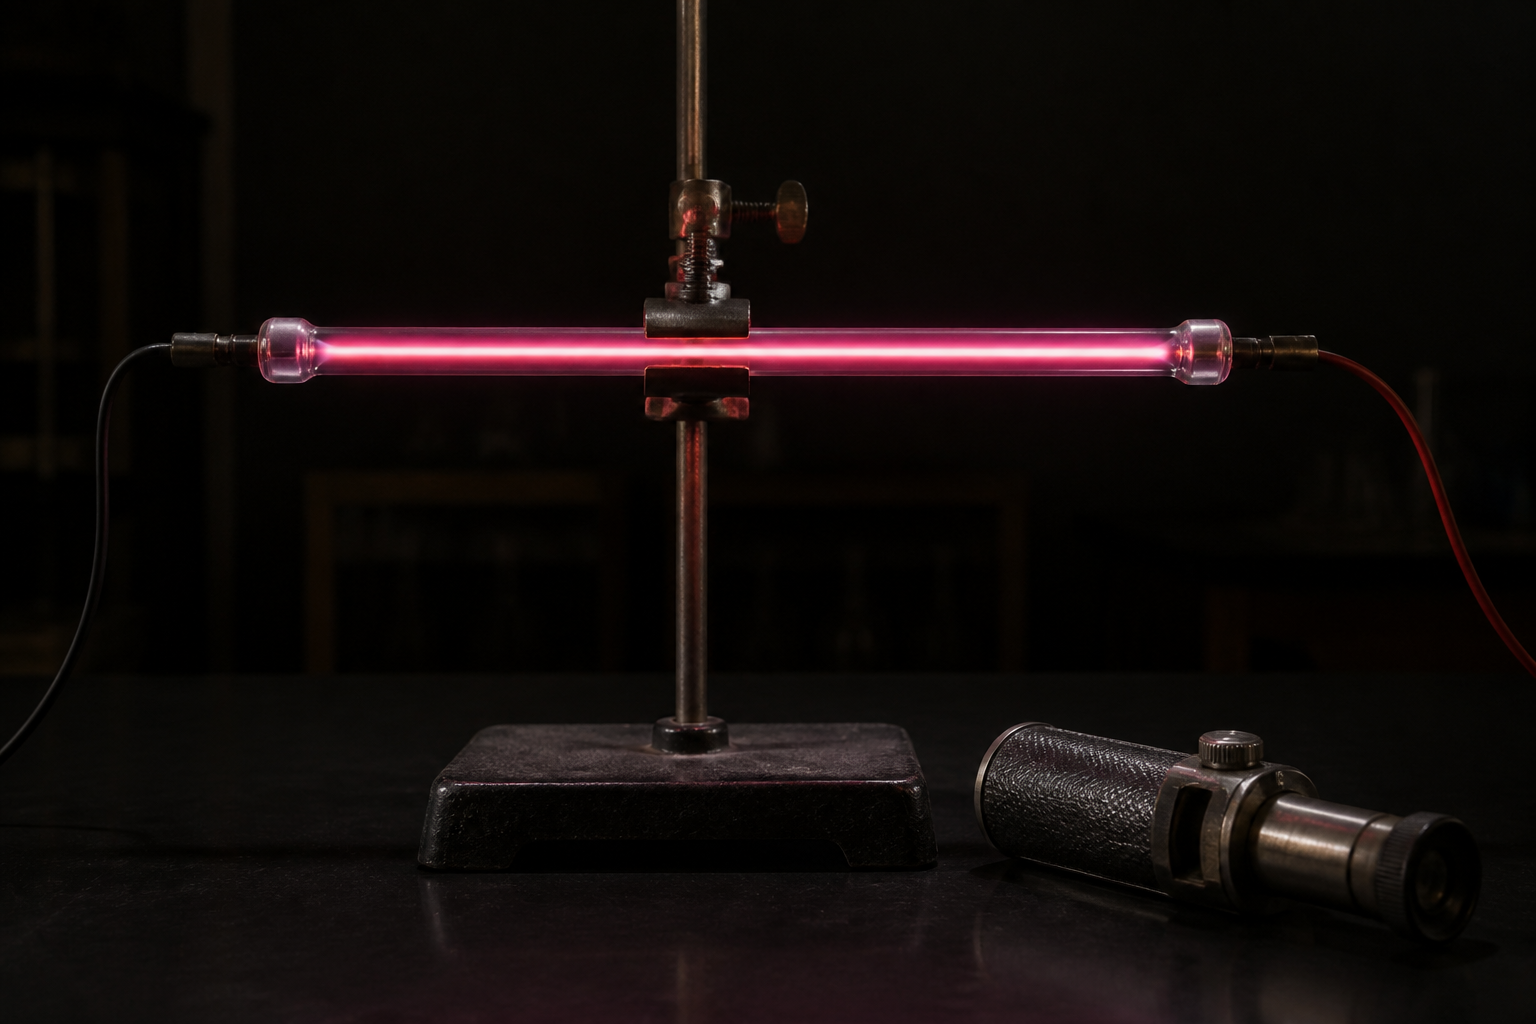
\includegraphics[width=0.58\linewidth]{images/book5/ai/b5-11-discharge-tube.png}

{\small Tabung lucutan hidrogen dan sebuah spektroskop saku: pijar merah mudanya, setelah terpilah, menjadi garis Balmer --- yakni sidik jari bilangan bulat yang diturunkan bab ini dari potensial Coulomb.}
\end{omfigure}

\section{Latihan}

\begin{exercise}[$\star$]\label{exo:b3:hydrogen-atom:1}
(a) Periksalah lewat penyulihan bahwa $u = Cr\eu^{-r/a_0}$ menyelesaikan
\omterm{prop:b3:schrodinger-three-dimensions:swave}{persamaan radial} $l = 0$ dengan $E = -E_{\text{I}}$, asalkan $a_0 =
\hbar^2/m_{\text{e}}k$. (b) Normalkanlah ($\int_0^\infty
x^2\eu^{-x}\dd x = 2$). (c) Periksalah dimensi $a_0$ dan
$E_{\text{I}}$. (d) Mengapa tak ada keadaan di bawah $-E_{\text{I}}$
(kemukakanlah dengan \cref{exo:b3:schrodinger-three-dimensions:12})?
\end{exercise}

\begin{exercise}[$\star$]\label{exo:b3:hydrogen-atom:2}
Hitunglah (a) panjang gelombang Lyman $\alpha$ dan batas Lyman; (b)
ketiga garis Balmer pertama beserta batas Balmernya --- yang mana yang
tampak, dan apa warnanya? (c) rentang deret Paschen; (d) frekuensi
transisi $n = 110 \to 109$.
\end{exercise}

\begin{exercise}[$\star$]\label{exo:b3:hydrogen-atom:3}
Untuk keadaan dasarnya: (a) tentukanlah maksimum $P_{1s}(r)$; (b)
hitunglah $\langle r\rangle$; (c) hitunglah peluang menemukan
elektronnya di luar $2a_0$ ($\int_x^\infty t^2\eu^{-t}\dd t = (x^2 +
2x + 2)\eu^{-x}$); (d) mengapa gambaran ``orbit'' berjejari tepat
$a_0$ menyesatkan?
\end{exercise}

\begin{exercise}[$\star$]\label{exo:b3:hydrogen-atom:4}
(a) Daftarkanlah pasangan $(l, m)$ untuk $n = 3$ lalu periksalah cacahnya $n^2 =
9$. (b) Dengan spinnya, berapa keadaan dalam kulit
$n = 1, 2, 3$? (c) Cocokkanlah dengan panjang $2, 8, 18$ baris tabel
berkalanya. (d) Degenerasi yang mana (dalam $m$, atau dalam $l$) yang
bertahan pada elektron terluar natrium, dan mengapa yang lain pecah?
\end{exercise}

\begin{exercise}[$\star\star$]\label{exo:b3:hydrogen-atom:5}
Tangga Moseley. Sebuah elektron dalam (kulit K) sebuah unsur $Z$
bergerak dalam medan inti yang nyaris telanjang, yang disaring satu
elektron K lainnya: muatan efektifnya $\approx Z - 1$. (a) Tunjukkanlah
bahwa energi sinar-X $2p \to 1s$ kira-kira $\tfrac34(Z-1)^2E_{\text{I}}$.
(b) Hitunglah untuk tembaga ($Z = 29$) lalu bandingkanlah dengan
K$\alpha$ terukur pada \qty{8.05}{keV}. (c) Moseley (1913) memetakan
$\sqrt{\nu}$ terhadap $Z$ dan memperoleh garis lurus: apa yang
dibuktikannya tentang makna nomor atom? (d) Ramalkanlah energi
K$\alpha$ unsur $Z = 43$ yang waktu itu belum ditemukan.
\end{exercise}

\begin{exercise}[$\star\star$]\label{exo:b3:hydrogen-atom:6}
Positronium. (a) Berilah alasan bagi $\mu = m_{\text{e}}/2$ lalu
berikanlah energi ikat dan \omterm{thm:b3:hydrogen-atom:levels}{jejari Bohrnya}. (b) Berapa panjang gelombang
Lyman $\alpha$-nya? (c) Para-positronium memusnahkan diri menjadi dua
foton: berapa energinya dan bagaimana arah nisbinya (dari
\cref{ch:b3:relativistic-dynamics})? (d) Di manakah kedokteran
mendeteksi sidik ini setiap hari?
\end{exercise}

\begin{exercise}[$\star\star$]\label{exo:b3:hydrogen-atom:7}
Eksiton. Dalam galium arsenida, $\varepsilon_{\text{r}} = 12.9$ dan
massa efektif tereduksinya $\mu = 0.058\,m_{\text{e}}$. (a) Tunjukkanlah
$a_{\text{ex}} = a_0\,\varepsilon_{\text{r}}\,m_{\text{e}}/\mu$ lalu
hitunglah. (b) Berapa energi ikat eksitonnya? (c) Bandingkanlah
$a_{\text{ex}}$ dengan jejari titik kuantum pada
\cref{pb:b3:schrodinger-three-dimensions:1} lalu berilah alasan,
akhirnya, bagi pengabaian suku Coulombnya pada titik yang kecil. (d)
Mengapa garis eksiton hanya muncul dalam semikonduktor yang \emph{murni
dan dingin} ($k_{\text{B}}T$ berbanding jawaban Anda pada (b))?
\end{exercise}

\begin{exercise}[$\star\star$]\label{exo:b3:hydrogen-atom:8}
Penembusan dan logam alkali. Natrium adalah elektron valensi mirip
hidrogen di luar teras tertutup bermuatan efektif $+e$.
(a) Manakah di antara $3s$, $3p$, $3d$ yang paling merasakan inti yang
tersaring tak sempurna, dan mengapa (ingatlah gambar radialnya)? (b)
Aras terukurnya adalah $E_{3s} = \qty{-5.14}{eV}$, $E_{3p} = \qty{-3.04}{eV},
E_{3d} = \qty{-1.52}{eV}$: periksalah bahwa $3d$ nyaris hidrogenik
($n = 3$) sedangkan $3s$ jauh lebih dalam, lalu jelaskanlah. (c)
Hitunglah panjang gelombang $3p \to 3s$: warna termasyhur apakah itu?
(d) Tuliskanlah aras alkalinya sebagai $-E_{\text{I}}/(n - \delta_l)^2$
lalu tariklah ``cacat kuantum'' $\delta_s$ dan $\delta_p$ untuk natrium.
\end{exercise}

\begin{exercise}[$\star\star$]\label{exo:b3:hydrogen-atom:9}
Sebuah proton dalam nebula menangkap sebuah elektron ke $n = 100$. (a)
Berapa energi yang dilepaskan dalam foton penangkapannya jika
elektronnya datang nyaris bebas? (b) Atomnya menuruni tangganya,
terutama lewat langkah $\Delta n = 1$ pada $n$ tinggi: pada pita mana
foton itu jatuh? (c) Langkah terakhir penurunannya adalah Lyman
$\alpha$; cahaya tampak nebula dikuasai H$\alpha$: telusurilah langkah
penurunan yang mana itu. (d) Jelaskanlah mengapa nebula pancaran
berpijar \emph{merah} padahal garis terkuat hidrogen (Lyman $\alpha$)
bersifat ultraungu.
\end{exercise}

\begin{exercise}[$\star\star\star$]\label{exo:b3:hydrogen-atom:10}
Rata-rata dan virialnya. Untuk keadaan dasarnya, hitunglah (a)
$\langle 1/r\rangle$ lalu periksalah $\langle E_p\rangle = -2E_{\text{I}}
= 2E_1$; (b) $\langle E_k\rangle = +E_{\text{I}}$, sehingga memeriksa
nisbah virial pada \cref{exo:b3:hamiltonian-mechanics:4}; (c) laju akar
rata-rata kuadrat elektronnya beserta $v/c$; (d) orde besar medan magnet yang dirasakan
\emph{protonnya} akibat gerak elektronnya (sebuah lingkar arus
$ev/2\pi a_0$ yang dilihat pada jarak $a_0$) --- sebuah bilangan yang
akan diperlukan struktur hiperhalus.
\end{exercise}

\begin{exercise}[$\star\star\star$]\label{exo:b3:hydrogen-atom:11}
Seberapa halus struktur halus itu. (a) Tunjukkanlah bahwa skala laju
keadaan dasarnya $\langle v^2\rangle^{1/2}/c = \alpha \approx 1/137$, dan
untuk $Z$ mirip hidrogen: $Z\alpha/n$. (b) Koreksi relativistiknya masuk
pada orde nisbi $(v/c)^2$: perkirakanlah skala struktur halusnya
$\alpha^2E_{\text{I}}$ dalam meV, beserta orde pembelahannya untuk
$n = 2$ dalam GHz. (c) Untuk uranium mirip hidrogen ($Z = 92$): berapa
$v/c$ pada $n = 1$ --- apakah perlakuan tak relativistiknya masih dapat
dipertahankan? (d) Apa yang diumumkan secara fisis oleh pembesaran tanpa
batas yang formal pada $Z\alpha \to 1$ ($Z \approx 137$)?
\end{exercise}

\begin{exercise}[$\star\star\star$]\label{exo:b3:hydrogen-atom:12}
Degenerasi yang tak masuk akal. (a) Dalam mekanika klasik, tunjukkanlah
bahwa untuk $V = -k/r$ orbitnya menutup (tanpa presesi) dengan mengutip
vektor kekal Laplace--Runge--Lenz $\vect A = \vect p\wedge\vect
L - mk\,\vect e_r$ --- periksalah $\dd\vect A/\dd t = 0$ dengan memakai
hukum Newton. (b) Kemukakanlah: sebuah vektor kekal yang menetapkan
sumbu elipsnya merupakan simetri tambahan di luar rotasinya --- dan
simetri tambahan berarti degenerasi tambahan (ingatlah
\cref{exo:b3:quantum-formalism:9}). (c) Tambahkanlah koreksi $1/r^2$
yang kecil pada potensialnya lalu tunjukkanlah bahwa elipsnya
berpresesi: sumbunya berputar, dan $\vect A$ tak lagi kekal. (d)
Kaitkanlah: dalam atom berelektron banyak potensial efektifnya bukan
$1/r$ murni, dan degenerasi $l$-nya pecah (natrium!); dalam hidrogen
sendiri, kerelatifan memasok koreksi kecilnya --- ciri teramati yang
mana pada \cref{exo:b3:hydrogen-atom:11} itu?
\end{exercise}

\section{Soal: Atom raksasa}

\begin{problem}[{Soal akhir pekan --- atom Rydberg, dari pijar radio
Galaksi sampai komputer kuantum}]\label{pb:b3:hydrogen-atom:1}
Regangkanlah hidrogen sampai $n \approx 100$ dan ia menjadi benda yang
berbeda jenisnya: selebar beberapa mikrometer, terikat oleh
milielektronvolt, luar biasa peka --- dan luar biasa berguna. Soal ini
menyekalakan penyelesaian hidrogennya ke atas, mula-mula ke awan
antarbintang yang bersiaran pada panjang gelombang sentimeter, lalu ke
larik laboratorium tempat raksasa semacam itu saling membelit menjadi
pengolah. Data:
$E_{\text{I}} = \qty{13.6}{eV}$, $a_0 = \qty{52.9}{pm}$,
$R_{\text{H}}c = \qty{3.29e15}{Hz}$, $k_{\text{B}}T$ pada
\qty{300}{K} adalah \qty{25.9}{meV}.

\medskip\noindent\textbf{Bagian I --- Hukum penyekalaannya.}
\begin{enumerate}
  \item Berikanlah keempat penyekalaan dasarnya terhadap $n$: ukuran
        $\langle
        r\rangle$, ikatan $|E_n|$, jarak aras $E_{n+1} - E_n$ (untuk
        $n$ besar), dan frekuensi orbit klasik orbit Bohr yang
        bersesuaian.
  \item Tunjukkanlah bahwa untuk $n$ besar frekuensi transisi $n+1 \to
        n$ mendekati $2R_{\text{H}}c/n^3$, lalu periksalah bahwa ia sama
        dengan frekuensi orbit klasiknya (asas korespondensi pada
        \cref{pb:b3:hamiltonian-mechanics:1}, yang kini lengkap).
  \item Hitunglah ukuran dan ikatannya pada $n = 50$ dan $n = 100$.
  \item Dipol listrik sebuah atom Rydberg berskala sebagai $n^2ea_0$:
        hitunglah pada $n = 50$ dalam debye ($1\,\text{D} =
        \qty{3.34e-30}{C.m}$) lalu bandingkanlah dengan \qty{1.85}{D}
        milik molekul air.
  \item Perkirakanlah medan listrik yang mencabik atom $n = 50$ itu,
        sebagai $F \sim |E_n|/(e\,\langle r\rangle)$, dalam V/cm.
  \item Mengapa atom semacam itu tidak dapat bertahan dalam kimia vakum
        laboratorium biasa --- namun bertahan baik-baik saja di ruang
        antarbintang (bandingkanlah laju tumbukannya)?
\end{enumerate}

\medskip\noindent\textbf{Bagian II --- Garis rekombinasi
Galaksi.}
Dalam nebula terionkan, proton menangkap elektron ke $n$ yang tinggi;
penurunannya memancarkan sisir ``garis rekombinasi radio''.
\begin{enumerate}[resume]
  \item Hitunglah frekuensi transisi $n = 110 \to 109$
        (yang disebut H109$\alpha$).
  \item Pada pita mana ia jatuh, dan teleskop macam apa yang
        menerimanya?
  \item Hitunglah panjang gelombang H109$\alpha$ lalu bandingkanlah
        dengan ukuran atom pemancarnya: berapa atom muat dalam satu
        panjang gelombang?
  \item Garis ini mengukur suhu nebulanya lewat lebar Dopplernya: pada
        $T = \qty{e4}{K}$, laju termal hidrogennya
        $\sim\qty{12.8}{km/s}$ --- hitunglah lebar garis pecahannya
        $\Delta\nu/\nu$ beserta lebar H109$\alpha$ dalam kHz.
  \item Gelombang radio menembus debu yang menghitamkan langit optis:
        apa yang karenanya dapat dipetakan para astronom garis
        rekombinasi yang tak dapat dipetakan astronom garis Balmer?
  \item Di atas kira-kira $n \sim 1000$ (atom selebar $0.05$ milimeter!),
        arasnya mengabur menjadi kontinum bahkan di angkasa:
        sebutkanlah dua efek yang melebarkan atau memusnahkan keadaan
        semacam itu.
\end{enumerate}

\medskip\noindent\textbf{Bagian III --- Raksasa di laboratorium.}
\begin{enumerate}[resume]
  \item Laser menggerakkan atom rubidium ke $n \approx 70$ dalam larik
        penjepit optis berjarak mikrometer. Dua atom semacam itu yang
        terpisah jarak $R$ berinteraksi lewat dipol imbasannya
        (ingatlah \cref{exo:b3:harmonic-oscillator:10}): dengan dipol
        $\propto n^2$, tunjukkanlah bahwa kekuatan van der Waalsnya
        berskala sebagai $n^{11}$ yang raksasa (pakailah
        $C_6 \propto d^4/\Delta E$ dengan jarak aras $\Delta E \propto n^{-3}$).
  \item ``Pemblokiran'': di dalam jejari $R_{\text{b}}$, interaksinya
        menggeser keadaan tereksitasi gandanya keluar dari resonansi
        lasernya, sehingga \emph{dua} atom tidak dapat sama-sama
        tereksitasi. Jelaskanlah dalam satu kalimat mengapa hal ini
        mewujudkan sebuah gerbang dua kubit.
  \item Jejari pemblokirannya mencapai beberapa mikrometer --- ribuan
        kali ukuran keadaan dasar atomnya: mengapa jangkauan yang
        panjang ini (bandingkanlah dengan jangkauan nanometer kimia)
        justru yang diinginkan sebuah pengolah yang dapat diperbesar?
  \item Keadaan Rydberg pada $n = 70$ hidup $\sim\qty{100}{\micro s}$
        sedangkan sebuah gerbang memakan $\sim\qty{0.5}{\micro s}$:
        kira-kira berapa operasi muat dalam satu umur, dan mengapa
        nisbah itu, bukan umurnya saja, yang berperan?
  \item Radiasi benda hitam suhu ruang, yang memuncak di dekat
        \qty{100}{meV} namun kaya akan ekor berenergi rendah,
        menggerakkan transisi antara aras Rydberg bertetangga yang
        hanya berjarak $\sim\qty{0.1}{meV}$: mengapa percobaan
        berketelitian tinggi harus mengurung atomnya dalam perisai
        dingin?
  \item Perkirakanlah berapa transisi dipol mirip antena ($\propto n^2$)
        yang digerakkan mandi foton \qty{300}{K} tiap sekon
        dibandingkan atom $n = 1$: penyekalaan yang mana yang menjadikan
        atom Rydberg \emph{sensor} medan gelombang mikro dan terahertz
        yang sangat halus?
\end{enumerate}

\medskip\noindent\textbf{Bagian IV --- Gambaran besarnya.}
\begin{enumerate}[resume]
  \item Satu rumus, $E_n = -E_{\text{I}}\mu Z^2/m_{\text{e}}n^2$,
        membentang berapa orde besar energi ikat dari uranium mirip
        hidrogen ($Z = 92$, $n = 1$) sampai ke keadaan Rydberg
        $n = 1000$? Hitunglah kedua ujungnya.
  \item Umur radiatif keadaan ber-$l$ rendah berskala sebagai $n^3$:
        dari umur $2p$ sebesar \qty{1.6}{ns}, perkirakanlah umur
        keadaan $100p$ --- lalu bandingkanlah dengan soal benda hitam
        suhu ruang pada Bagian III.
  \item Di CERN, antiatom antihidrogen kini dispektroskopi pada selang
        $1s \to 2s$ sampai lima belas angka: simetri dasar apa yang
        diuji kesesuaiannya dengan hidrogen biasa, dan mengapa hidrogen
        adalah atom yang tepat untuk perbandingan itu?
  \item Pada $n \sim 100$ gelombang de Broglie elektronnya membungkus
        orbit yang nyaris klasik; pada $n = 1$ sama sekali tak ada
        orbit: dalam satu kalimat, di manakah gambaran klasiknya
        menyala?
  \item Tetapan Rydberg diukur sampai lima belas angka: mengapa
        hidrogen, di antara semua sistem, merupakan jangkar ketelitian
        yang wajar bagi fisika atom?
  \item Hadiah Nobel 2012 (Haroche) memakai atom Rydberg sebagai
        pencacah foton yang tidak memusnahkan fotonnya: dua sifat mana
        dari Bagian I dan III yang menjadikannya penyelidik nirbongkar
        yang ideal bagi medan gelombang mikro?
  \item Ringkaslah hasil bernama itu: penyekalaan $n^2$, $n^{-2}$,
        $n^{-3}$ dan $n^{11}$ satu atom yang terselesaikan secara eksak
        meregangkan hidrogen dari \qty{52.9}{pm} sampai setengah
        mikrometer, menala suaranya dari \qty{121.6}{nm} sampai
        \qty{6}{cm}, dan menjadikannya sekaligus mercusuar radio
        Galaksi dan gerbang dua kubit komputer kuantum atom netral.
\end{enumerate}
\end{problem}
